\documentclass[11pt]{article}
\usepackage[a4paper,margin=26mm]{geometry}
\usepackage{amsmath,amssymb,amsthm,mathtools,booktabs,microtype}
\usepackage{tikz}
\usetikzlibrary{arrows.meta,positioning}
\usepackage[hidelinks]{hyperref}
\newtheorem{theorem}{Theorem}
\newtheorem{lemma}[theorem]{Lemma}
\newtheorem{corollary}[theorem]{Corollary}
\newtheorem{proposition}[theorem]{Proposition}
\theoremstyle{definition}\newtheorem{definition}[theorem]{Definition}
\newcommand{\HH}{\mathcal H_W}
\newcommand{\RR}{\mathcal R_T}
\newcommand{\sym}{\mathbin{\triangle}}
\newcommand{\N}{\mathbb N}
\newcommand{\Z}{\mathbb Z}
\newcommand{\COne}{C_1(T)}
\newcommand{\CAll}{C_{\mathrm{all}}(T)}
\title{When to Intervene:\\Predictive Memory in a Langton Highway}
\author{Hao Ke}
\date{}
\begin{document}
\maketitle
\begin{abstract}
How much of a self-written environment must a predictive state retain when a
simple observation is supplemented by a local intervention? We answer this
question for one exact standard-highway trace of the classical Langton ant.
Every source has finite black support and the same complete uncontrolled future.
Nevertheless, predicting the first $T$ turns for every possible time of a single
current-cell toggle requires $\Theta(T^2)$ source-dependent bits in the worst
case. An explicit matrix of protected readout lanes gives the lower bound:
the chosen intervention time selects one row, which is read autonomously before
permanent standard-highway recovery. The construction retains the entire field,
has word-independent mass and signed row/column charges, and admits exact
finite-horizon response counts. More generally a menu of at most $q\le T$
possible trigger times requires $\Theta(qT)$ bits, uniformly for large $T$. Arbitrary further toggles do not increase the
quadratic order; their exact quotient is determined by the free colors in an
alternating-axis causal region. A binary-entropy argument preserves the quadratic
lower bound under a specified nonzero prediction error. The result distinguishes
predictive storage from execution time and passive regularity from sufficiency
under future interaction.
\end{abstract}

\section{A predictive state depends on the allowed experiment}
A finite moving controller can use its environment as memory by writing it and
subsequently revisiting it. A periodic observed motion need not make all of that
memory irrelevant to future interventions. This raises a concrete compression
question: how many distinctions in the microscopic source must be retained
\emph{before} the next experimental choice is known?

Gajardo, Moreira and Goles established finite circuit calculation by the
classical ant~\cite{gmg}.
Input-conditioned predictive equivalence is likewise central to the theory of
$\epsilon$-transducers \cite{bc}. Our setting is different from a stationary
stochastic channel: it is a deterministic, finite-source, finite-horizon
worst-case problem with one explicitly constrained physical intervention.

We fix the ant at the origin facing east. White cells turn it right and become
black; black cells turn it left and become white; it then moves one unit.
A complete state includes the entire finite black set, not an active-core
approximation. At pre-update time $t$, the experimenter may toggle the cell
currently occupied by the ant, immediately before its ordinary update. No
remote edit, head repositioning, or later boundary operation is implicit.

Fix a standard 104-turn phase $W$, specified in Section~\ref{sec:seeds}. Let
$\HH$ be the class of all finite black fields whose whole uncontrolled turn
stream is $W^\omega$. With a common initial pose, the turn stream determines
the position and heading trace. Thus every member of $\HH$ is indistinguishable
by \emph{infinite passive observation}, not only by an observed finite prefix.

For a horizon $T$, let $C_1(T)$ count distinct response maps on $\HH$ when the
permitted controls are no intervention or a single toggle at any $s<T$.
Let $C_{\mathrm{all}}(T)$ permit an arbitrary binary toggle word of length $T$.
Each response consists of the first $T$ turn letters. A sufficient summary is
prepared from the microscopic input \emph{before} the control is specified;
its decoder receives that control but cannot reread the discarded field.
The minimal fixed-length exact storage is the ceiling of the logarithm of the
number of response maps.

\begin{theorem}[Quadratic one-intervention storage]\label{th:main}
As $T\to\infty$, $\log_2 C_1(T)=\Theta(T^2)$. More explicitly, for $T\ge74$, put
\[
a=\left\lfloor\frac{T-70}{4}\right\rfloor,
\qquad n=1+\left\lfloor\frac{a-1}{78}\right\rfloor.
\]
Then
\begin{equation}\label{eq:main}
na-39n(n-1)\ \le\ \log_2 C_1(T)\ \le\ \frac{T(T-1)}2.
\end{equation}
The lower bound is $T^2/2496+O(T)$. Its witnesses fit in a square of side $O(T)$,
use $O(T^2)$ black cells, and recover a certified standard highway after every
scheduled intervention used in the lower-bound proof.
\end{theorem}

For one prescribed intervention time, the same task has linear storage
order. Allowing the time to select a channel changes the prediction problem.

\begin{theorem}[Exact complete-control quotient]\label{th:all}
Let $D$ be the entire read footprint of $W^\omega$, and let $\RR$ be the set of
sites a turn-at-every-step head can read before time $T$. Then
\[
C_{\mathrm{all}}(T)=2^{|\RR\setminus D|}.
\]
For $T\ge13$, with $r=T\bmod4$,
\begin{equation}\label{eq:all}
\log_2 C_{\mathrm{all}}(T)
=T^2-T+1-22\lfloor T/4\rfloor+b_r,
\qquad (b_0,b_1,b_2,b_3)=(33,27,22,16).
\end{equation}
\end{theorem}

Thus one selected-time toggle already attains the spatial quadratic order
available under arbitrary toggling. It does not attain all the same responses
or the same leading constant. This separates a nearly trivial passive
predictor from a large counterfactual response table in the same dynamics.

\section{Two standard seeds and a certified activation port}\label{sec:seeds}
Number headings $N,E,S,W$ by $0,1,2,3$. The two thirteen-cell fields are
\begin{align*}
P={}&\{(0,-3),(0,-2),(0,-1),(1,-2),(2,-2),(2,0),(3,-3),\\
 &\hspace{12mm}(3,0),(4,-3),(4,-1),(5,-2),(5,-1),(6,-1)\},\\
Q={}&\{(0,2),(0,3),(1,0),(1,4),(1,5),(1,6),(2,0),\\
 &\hspace{12mm}(2,1),(2,2),(2,5),(3,0),(3,3),(3,4)\}.
\end{align*}
For complete reproducibility, $W$ is the concatenation of these four lines:
\begin{center}\small\ttfamily
RLRLLRRRRLLRLLRRRRLLRRRRLL\par
RLRRRRLRLLLLRRRRLRRLRRRRLL\par
LLRLRRRRLRRRRLLLLRLRRRRLRL\par
LRRLLLLRRLLRRRRLLRRLRLLRLL
\end{center}
The executable certificate stores and checks the literal word of length 104.
The word in the displayed line wrapping is also checked against that source.

The seed $P$ from heading $E$ executes $W^\omega$ with displacement $(2,-2)$
per period. Its period reads satisfy $-4\le x+y\le6$ and $0\le x\le8$.
The seed $Q$ from the origin with heading $N$ executes the same word with displacement $(2,2)$.
Its infinite read footprint has
\begin{equation}\label{eq:outguard}
x\ge0,\qquad y\ge0,\qquad -4\le y-x\le6.
\end{equation}
Every cell of $Q$ has $x\le3$ and $y-x\le5$.

We explain why these are finite proof obligations. Group period reads as
$q_i=c+k_i d$ modulo the full drift $d$. A fixed cell $c+z d$ is read by precisely
the phases with $k_i\le z$, in increasing order of $104z+i-104k_i$. The requested
letters must alternate. Eligible lists change only at the finitely many $k_i$.
Their first letters specify the initial colors; the final infinite interval
must begin with $R$. The check reconstructs the exact finite seed, rather than
merely finding a repeated finite trace. Each seed has 22 classes and 130 adjacent
letter comparisons. Cellwise alternation followed by induction over physical
time establishes the infinite execution. Section~\ref{sec:verification} describes
the independent reconstructions.

At phase 72 of the $P$ execution the pose is $(8,-2),E$ and the ordinary turn is
$R$. The pre-update toggle makes that cell black. The ordinary update then turns
left and restores the cell to white, leaving the head at $(8,-1),N$ and the
pre-update background unchanged.
There is one important boundary exception. The possible next left turn reads
$(7,-1)$, whose coordinate sum is 6 rather than 7. This cell is not in $P$ and
not among its first 72 reads. In period $a$, a read of its translate by an earlier
period $b<a$ would require phase $x$-coordinate $7+2(a-b)\ge9$, exceeding the
period maximum 8. It is consequently white at activation for every $a\ge0$.
This check is essential: a bare half-plane argument would not suffice.

\section{Protected time-addressed data channels}
For $b\in\{0,1\}$ define binary tiles and their exact outputs by
\[
A_0=\{1,2\}\times\{0,1\},\quad A_1=\{0,3\}\times\{0,1\},
\]
\[
A'_0=\{0,2\}\times\{0,1\},\quad A'_1=\{-1,3\}\times\{0,1\}.
\]
From $(0,0),N$, the complete four-update identities are
\begin{equation}\label{eq:tiles}
A_0\xrightarrow{RLLR}A'_0,\qquad
A_1\xrightarrow{LRRL}A'_1,
\end{equation}
with common final pose $(0,2),N$. Reads stay in
$\{-1,0,1\}\times\{0,1\}$. Each source has four black cells and contributes
zero to every checker-signed row and column sum. The simultaneous protected placement of these tiles and seeds supplies
independent channels inside a single passive class.

For integers $n,m\ge1$ and a binary matrix $U=(u_{jr})_{0\le j<n,0\le r<m}$,
put
\[
s_j=312j+72,\qquad q_j=(8+6j,-1-6j),\qquad c_j=q_j+(0,2m),
\]
and define the complete source
\begin{equation}\label{eq:source}
B_U=P\ \cup\ \bigcup_{j<n}(Q+c_j)
\ \cup\ \bigcup_{j<n}\bigcup_{r<m}(A_{u_{jr}}+q_j+(0,2r)).
\end{equation}
All other cells are white. The unions are disjoint and
\begin{equation}\label{eq:mass}
|B_U|=13+n(13+4m).
\end{equation}
For fixed dimensions every source has the same bounding rectangle
$[0,6n+5]\times[\min(-3,5-6n),2m+5]$ and the same signed sum on each row and column.

\begin{figure}[t]
\centering
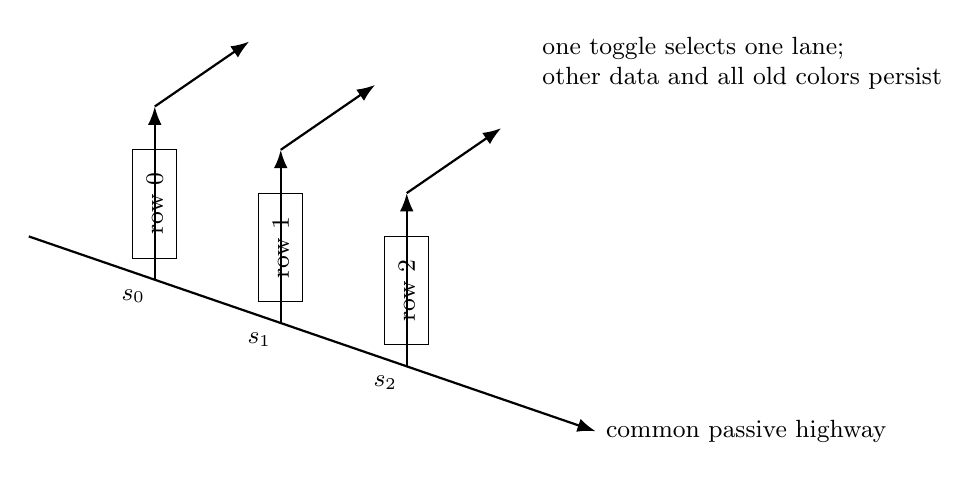
\begin{tikzpicture}[x=.8cm,y=.55cm,>=Latex,font=\small]
\draw[->,thick](-1,0)--(8,-4.5)node[right]{common passive highway};
\foreach \x/\y/\lab in {1/-1/0,3/-2/1,5/-3/2}{
 \draw[->,thick](\x,\y)--(\x,4+\y);
 \draw(\x-.35,\y+.5)rectangle(\x+.35,\y+3.0);
 \node[rotate=90]at(\x,\y+1.75){row \lab};
 \draw[->,thick](\x,\y+4)--(\x+1.5,\y+5.5);
 \node[below left]at(\x,\y){$s_{\lab}$};
}
\node[align=left,anchor=west]at(7,4){one toggle selects one lane;\\other data and all old colors persist};
\end{tikzpicture}
\caption{Schematic only. Exact coordinates and guards are in
\eqref{eq:source} and Lemma~\ref{lem:readout}. No physical run reads all lanes.}
\end{figure}

\begin{lemma}[Exact complete-field readout]\label{lem:readout}
Every $B_U$ belongs to $\HH$. If its only toggle occurs at $s_j$, its entire
turn stream is
\begin{equation}\label{eq:stream}
W^{3j}W_{0:72}\,L\,c(u_{j0})\cdots c(u_{j,m-1})\,W^\omega,
\qquad c(0)=RLLR,\quad c(1)=LRRL.
\end{equation}
At time $s_j+1+4r$, the pose is $q_j+(0,2r),N$. The complete field consists of
the passive $P$ field at time $s_j$, every cap and every nonselected data lane,
and the selected lane with each tile $k<r$ replaced by $A'_{u_{jk}}$.
Its first permanent standard entry is $s_j+4m+1-u_{j,m-1}$.
\end{lemma}
\begin{proof}
All added source cells have $x+y\ge7$, while every passive read has $x+y\le6$.
A first-difference induction proves passive agreement and retains all added
cells. At activation, Section~\ref{sec:seeds} supplies the northward entry and
its single boundary-cell guard. The selected lane reads only $x$ between
$q_j.x-1$ and $q_j.x+1$. Other source lanes have $x$ between $q_l.x$ and $q_l.x+3$;
spacing six separates them, since $3-6<-1$. Each tile reads its own two rows.
Induction using \eqref{eq:tiles} gives the exact checkpoints and arrives at $c_j$.

It remains to prove infinite protection, not just arrival at a seed. The outgoing
$Q$ reads have $x+y\ge7+2m$, so cannot meet the passive background. Selected-lane
residues have $y<c_j.y$. Every earlier lane has $x\le c_j.x-3$, whereas the
outgoing reads have $x\ge c_j.x$. For $l>j$, a cap cell has
\[
y-x\le c_l.y-c_l.x+5
=c_j.y-c_j.x-12(l-j)+5\le c_j.y-c_j.x-7,
\]
below the outgoing lower bound $c_j.y-c_j.x-4$. Later-lane data satisfy the
stronger upper bound $c_j.y-c_j.x-13$. Thus all complete residual fields are
unread by the whole outgoing standard tail.

The word $W$ is primitive and ends in $LL$. At the cap boundary its phase is
fixed by the infinite suffix. If the final bit is zero, its code ends in $R$,
so the preceding letter disagrees with that phase. If the final bit is one,
its last $L$ agrees but its penultimate $R$ does not. These give the two first-entry
times asserted. No unrelated shorter phase can agree forever with a primitive
104-period suffix.
\end{proof}

\section{Counting exactly the visible information}
The first symbol encoding bit $u_{jr}$ occurs at update $s_j+1+4r$. Thus exactly
\begin{equation}\label{eq:q}
q_j(T)=\min\!\left(m,\max\!\left(0,
\left\lfloor\frac{T-s_j+2}{4}\right\rfloor\right)\right)
\end{equation}
bits are visible in the $T$-turn response to $s_j$.

\begin{proposition}\label{prop:profile}
For the scheduled experiment set consisting of no toggle and the $n$ times
$s_j$, the exact number of response maps on \eqref{eq:source} is
$2^{Q(n,m,T)}$, where $Q(n,m,T)=\sum_{j<n}q_j(T)$.
\end{proposition}
\begin{proof}
The response to $s_j$ depends on no other data row. A first differing visible
bit changes the first letter of its four-step code and therefore the observed
trace. Conversely, bits after the visible prefix cannot affect that response.
Every assignment to the visible prefixes occurs, proving both bounds.
\end{proof}

Choose $m=a$ and $n$ from Theorem~\ref{th:main}. Then $q_j=a-78j>0$ for
$0\le j<n$, and summing gives the lower bound in \eqref{eq:main}. The scheduled
controls are only a subset of all one-toggle controls, so additional controls
cannot remove distinctions. Since $n=a/78+O(1)$ and $a=T/4+O(1)$, the exponent
is $T^2/2496+O(T)$. Equation~\eqref{eq:mass} and the bounding rectangle give the
resource assertions.

For the upper bound, the response to a toggle at $s$ shares the fixed first $s$
passive letters, has the forced opposite letter at $s$, and has at most $T-s-1$
free binary letters afterwards. Multiplying the possibilities over all $s$ gives
\[
C_1(T)\le\prod_{s=0}^{T-1}2^{T-s-1}=2^{T(T-1)/2}.
\]
This does not assume those putative tables are all physically realizable.
It completes Theorem~\ref{th:main}. For the single prescribed time 72 the upper
bound is $T-73$ bits; one lane with sufficiently many bits gives a lower bound
$\lfloor(T-70)/4\rfloor$. Therefore its growth order is linear.

The summary must support an experiment chosen \emph{after} it is prepared.
If the intervention time is known during encoding, only its row need be saved.
An individual experiment outputs only $O(T)$ information-bearing symbols.
The quadratic theorem concerns the family of counterfactual responses, not
information manufactured by a single toggle.

\section{How the timing menu controls storage}\label{sec:menu}
For a menu $A\subseteq\{0,\ldots,T-1\}$ let $b(T,A)$ be the ceiling of the
binary logarithm of the number of distinct response tables on $\HH$ for the
single-toggle experiments indexed by $A$. Define
\[
 M(T,q)=\max_{|A|\le q}b(T,A),\qquad 1\le q\le T.
\]
The encoder knows the menu but must store its summary before the particular
experiment is chosen. In particular $M(T,T)=\lceil\log_2 C_1(T)\rceil$.

\begin{theorem}[Uniform timing-menu law]\label{th:menu}
For $T\ge832$ and $1\le q\le T$,
\[
 \min\{q,\lfloor T/832\rfloor\}\lfloor T/8\rfloor
 \le M(T,q)\le qT-\frac{q(q+1)}2.
\]
Consequently $M(T,q)=\Theta(qT)$ with absolute constants uniform in this range.
\end{theorem}
\begin{proof}
A response for time $s$ has at most $T-s-1$ free letters. Summing over a menu
of at most $q$ times is bounded by the sum for $s=0,\ldots,q-1$, giving the
integer upper bound, including the ceiling in the definition of $b$.
For the lower bound use the already proved protected construction with
$n=\min(q,\lfloor T/832\rfloor)$ lanes and $m=\lfloor T/8\rfloor$ bits per lane.
The last lane reaches its cap at
\[
 312(n-1)+72+4m+1=312n+4m-239<T.
\]
Every one of the $nm$ bits therefore appears in its registered response.
Proposition~\ref{prop:profile} supplies exactly $2^{nm}$ distinct tables.
Finally $\lfloor T/832\rfloor\ge T/1664$ and $\lfloor T/8\rfloor\ge T/16$;
since $q\le T$, the lower bound is at least $qT/26624$.
\end{proof}

The same protected array thus connects the linear prescribed-time regime to
the quadratic unrestricted-time regime. The tighter construction of
Theorem~\ref{th:main} improves the explicit full-menu coefficient.

\section{Causal geometry and the exact unrestricted quotient}
After $t$ updates, a head initially facing east has made
$H_t=\lfloor t/2\rfloor$ horizontal and $V_t=\lceil t/2\rceil$ vertical moves.
Each sign on the next axis can be selected by a suitable current-cell toggle.
The reachable sites at that time are exactly
\[
K_t=\{-H_t,-H_t+2,\ldots,H_t\}\times
    \{-V_t,-V_t+2,\ldots,V_t\}.
\]
The coordinate parity classes for $t\bmod4=0,1,2,3$ are respectively
$(0,0),(0,1),(1,1),(1,0)$. Since $K_t\subset K_{t+4}$, the union
$\RR=\bigcup_{t<T}K_t$ contains only the last at most four rectangles.
Summing their sizes gives
\begin{equation}\label{eq:cone}
|\RR|=T^2-T+1\quad(T\ge1).
\end{equation}

\begin{lemma}[Exact controlled distinguishability]\label{lem:cone}
Two fields at the common initial pose give identical $T$-turn responses to all
binary control words if and only if their initial colors agree on $\RR$.
\end{lemma}
\begin{proof}
Agreement on $\RR$ persists while both heads read the same current site and
receive the same toggle. Every read before $T$ is in $\RR$, proving sufficiency.
Conversely choose a turn path reaching a differing site before $T$. Compute the
control word that forces the first field to follow that path. If the two executions
meet a difference earlier, their turns already separate. Otherwise their colors
at the chosen site differ, so the common control still gives opposite turns.
This proves necessity without assuming that an uncontrolled ant visits the site.
\end{proof}

Over all complete finite fields, every assignment on $\RR$ is possible.
Lemma~\ref{lem:cone} therefore also gives the exact general controlled quotient
$2^{T^2-T+1}$. The fixed passive class has fewer degrees of freedom because its
entire uncontrolled footprint has prescribed initial colors.

The first-difference argument identifies that full passive class:
\begin{equation}\label{eq:class}
\HH=\{P\cup A:A\text{ is a finite subset of }\Z^2\setminus D\}.
\end{equation}
Necessity follows from the required initial color at each first read on $D$;
sufficiency follows by induction, since the difference is never read. The
periodic certificate gives $P\subset D$. Every assignment to $\RR\setminus D$
therefore extends to a source in $\HH$. Lemma~\ref{lem:cone} proves
$C_{\mathrm{all}}(T)=2^{|\RR\setminus D|}$.

For the exact count, $D$ is the disjoint union of rays $b+\N(2,-2)$ with bases
\begin{align*}
&(0,-4),(0,-3),(0,-2),(0,-1),(0,0),\quad
(1,-5),(1,-4),(1,-3),(1,-2),(1,-1),\\
&(2,-1),(2,0),(3,-2),(3,-1),(3,0),(4,-1),(5,-1),\\
&(6,-2),(6,-1),(7,-2),(7,-1),(8,-2).
\end{align*}
For a base $(x,y)$, take the last $t<T$ of its parity class and set
$H=\lfloor t/2\rfloor,V=\lceil t/2\rceil$. Its intersection count is zero for
$t<0$, and otherwise equals
\begin{equation}\label{eq:ray}
\max\{0,1+\min(\lfloor(H-x)/2\rfloor,\lfloor(V+y)/2\rfloor)\}.
\end{equation}
All bases have $x\ge0,y\le0$, so no positive lower ray-index constraint appears.
For $T=13,14,15,16$ every inner minimum is at least $-1$. Increasing $T$ by four
increases both floors by one, and hence each ray count by one forever. The four
initial sums give $|\RR\cap D|=22\lfloor T/4\rfloor-b_{T\bmod4}$.
Together with \eqref{eq:cone}, this proves \eqref{eq:all}. This stabilization is
an explicit arithmetic induction, not a fit to a finite time sequence.

\section{Robustness to prediction error}
The exact counting theorem has an information-theoretic strengthening.
Write $h_2(p)=-p\log_2p-(1-p)\log_2(1-p)$ for binary entropy, with
$0\log_2 0=0$.
Fix the visible bits in Proposition~\ref{prop:profile}, randomize those $Q$ bits
independently and uniformly, and fix all other bits. Let $R$ be shared randomness
independent of the source, and let $M$ be a summary of at most $b$ bits. A query
selects one visible bit, equivalently its lane intervention and code-symbol time.

\begin{proposition}\label{prop:error}
If a decoder given $M,R$ and the query index predicts that symbol with average
bit error $\epsilon<1/2$, then
\[
b\ge Q\bigl(1-h_2(\epsilon)\bigr).
\]
\end{proposition}
\begin{proof}
Let $e_i$ be the error for bit $i$. Binary conditional entropy and concavity give
\[
H(U\mid M,R)\le\sum_i H(U_i\mid M,R)
\le\sum_i h_2(e_i)\le Qh_2(\epsilon).
\]
Since $H(U\mid R)=Q$ and $H(M\mid R)\le b$, subtracting the conditional entropy
proves the result. Independent decoder randomness may be included in $R$.
\end{proof}

The entropy argument is standard. The physical construction makes the requested
binary symbols genuine ant observations under the same one-toggle protocol.
This statement does not assume stochastic microscopic dynamics, a thermodynamic
entropy, or robustness to arbitrary noise in the lattice.

\section{Verification and reproducibility}\label{sec:verification}
The implementation uses only Python's standard library and a C++17 compiler.
Python uses vector rotations and coordinate sets. The native implementation uses
heading indices and independently normalizes full-drift classes; both reconstruct
the two infinite periodic seeds. Local checks verify the binary tile fields,
the phase-72 boundary exception, and the six strict separation inequalities used
in the all-parameter proof. The exact quotient count is reduced to its 22 rays
and four stabilization residues.

Matched full-field execution checks cover 1,474 matrices, 3,874 native runs and
2,276,414 updates per implementation, supplemented by 490 complete intermediate
checkpoints, 410 response-profile counts and 3,838 first-entry checks. Independent
controls retain unread cells at coordinate scale $10^{60}$ and reject corrupted
period seeds, remote future blockers and resource-cap misuse. These controls
supplement the analytic induction; they do not substitute for its unbounded
quantifiers. The source-bound report is rebuilt and compared without overwriting
its frozen data by
\begin{center}\small\ttfamily
python intervention\_capacity/reproduce.py
\end{center}
The computational trusted base includes both programs and their runtimes; no
formal proof assistant is assumed.

\section{Limitations}
The results concern source-dependent summary size. The initial matrices are
installed data of growing size. The theorems do not
claim unbounded information generation from one fixed finite seed, nor an
infinitely self-renewing controller. Every scheduled witness response recovers a
standard highway, but recovery after every \emph{unscheduled} toggle is not
asserted. The general finite-horizon quotient is defined regardless of any
unknown long-term fate. The sharp quadratic coefficient and the behavior after unscheduled toggles
remain open within this model.

The main distinction is nonetheless exact. A fixed periodic passive motion can
leave an area-sized amount of source information potentially relevant. One
experimental choice, its time rather than a sequence of steering commands, can
select enough independent readout channels to force quadratic predictive storage.
The result does not invalidate macrostate descriptions; it specifies the
observation and intervention contract under which one such description must grow.

\paragraph{Assistance and reproducibility.}
Proof development, exposition and verification code were assisted by ChatGPT.
The complete coordinate constructors, finite periodic obligations, independent
checker and frozen report accompany the source. The counting and information
inequalities are presented separately from the ant-specific embedding so their
logical dependencies can be audited.

\begin{thebibliography}{9}
\bibitem{gmg} A. Gajardo, A. Moreira and E. Goles.
Complexity of Langton's Ant.
\emph{Discrete Applied Mathematics} 117 (2002), 41--50.
\href{https://doi.org/10.1016/S0166-218X(00)00334-6}{doi:10.1016/S0166-218X(00)00334-6}.
Author version \href{https://arxiv.org/abs/nlin/0306022}{arXiv:nlin/0306022}.
\bibitem{bc} N. Barnett and J. P. Crutchfield.
Computational Mechanics of Input--Output Processes: Structured Transformations
and the $\epsilon$-Transducer.
\emph{Journal of Statistical Physics} 161 (2015), 404--451.
\href{https://doi.org/10.1007/s10955-015-1327-5}{doi:10.1007/s10955-015-1327-5}.
\end{thebibliography}
\end{document}
